
\documentclass[12pt,letterpaper]{article} 
\usepackage[letterpaper,left=3.5cm,right=3.5cm, top=3.0cm, bottom=3.0cm, footnotesep=1.0cm]{geometry} 
\usepackage{mathptmx}
\DeclareMathAlphabet{\mathcal}{OMS}{cmsy}{m}{n}
\usepackage[onehalfspacing]{setspace} 
\usepackage{fancyhdr} 
\usepackage{relsize}

\usepackage[bottom]{footmisc}
\usepackage{tabularx}
\usepackage{mathtools}
\pagestyle{empty}        


\usepackage{booktabs}    
\usepackage{natbib}      
\usepackage{bibentry}   

\usepackage{acronym}
\usepackage{multicol}

\usepackage{amsmath}
\usepackage{amssymb}
\usepackage{mathrsfs}
\usepackage{listings}
\usepackage{graphicx}
\usepackage{mathtools}
\usepackage[usenames,dvipsnames]{color}
\usepackage{hyperref}
\usepackage{caption}
\usepackage{subcaption}
\usepackage[section]{placeins}

\lstset{
  basicstyle=\scriptsize\ttfamily,
  stringstyle=\color{ForestGreen},
  morekeywords={real,vector, int, matrix},
  deletekeywords={data,frame,length,as,character},
  keywordstyle=\color{blue},
  commentstyle=\color{ForestGreen},
}

\numberwithin{equation}{subsection}

\begin{document}

\begin{center}\uppercase{Ludwig-Maximilians-University Munich}\end{center}
\begin{center}\uppercase{Department of Statistics}\end{center}

\vspace{3cm}

\title{Variable selection using grouped horseshoe priors}
\date{\vspace{-5ex}}
{\let\newpage\relax\maketitle}
\thispagestyle{empty}


\begin{center}
  \begin{large}
    \begin{Large}
      Bachelor's Thesis\\
    \end{Large}
    Department of Statistics  \\
  \end{large}
\end{center}
\begin{center}
  Author:\\
  \begin{large}
    Tobias Pielok\\
  \end{large}
\end{center}
\vspace{1cm}
\begin{center}
  \begin{large}
    Supervisor: Dr. Fabian Scheipl
  \end{large}
\end{center}

\begin{center}  \begin{large}
    Submission date: \\%\date{\today} \\
  \end{large}
\end{center}

\vspace{1,5cm}

\begin{center}
  \begin{large}
    \author{Tobias Pielok, B.Sc. (TUM)}\\
 \end{large}
  Marchgrabenplatz 5\\ 
  80805 Munich\\ 
  \url{t.pielok@campus.lmu.de}\\
  Matrikelnr.:  11381351\\
\end{center}

\newpage
\section*{Acknowledgement}
To Fabian Scheipl, for giving me the opportunity to write about such an interesting topic and great support. \\ \\
To my parents, for always believing in me.

\newpage
\setcounter{page}{1}
\tableofcontents
\newpage


\pagestyle{fancy}
\fancyhf{}
\fancyhead[R]{\thepage}
\renewcommand{\headrulewidth}{0pt} 
\section*{Notation and Symbols}

\begin{tabular}{lll}
$\mathcal{B}_\mathcal{M}\bigotimes\mathcal{B}_\mathcal{N}$ & & product-$\sigma$-algebra generated by $\{M\times N :\; M\in\mathcal{B}_\mathcal{M}, N\in\mathcal{B}_\mathcal{N} \}$ \\
$\theta \in \mathbb{R}^d$ & & If $\theta$ is a random variable: $\theta$ maps to $\mathbb{R}^d$ \\
$\text{C}^+(0,a)$ & & standard half-Cauchy distribution on the positive reals with scale parameter a
\end{tabular}

\pagebreak
\section{Introduction}
% need of variable selection -> what is variable selection
Often in data analysis the situation arises where not all parameters of a model can be well identified through the data. In these situation one possible way to estimate the model is via variable selection, which is a process where a subset of the most informative predictors is chosen, s.t. for this subset the model can be estimated for. \\ 
Variable selection can be carried out with a frequentist approach, e.g. lasso feature selection, or a Bayesian approach with so-called shrinkage priors. The most popular shrinkage priors are the spike-and-slab priors and the horseshoe priors. By using the horseshoe priors one applies global shrinkage to all variables, but allows for informative variables to locally escape the shrinkage. In this thesis the horseshoe priors are extended to the case of variables, which posses a grouped structure. Hence the priors are denoted as \textit{grouped horseshoe priors}. In section (\ref{sec:basics}) the Bayesian inference of the grouped horseshoe priors is rigorously introduced, and how this inference can it be executed computationally. In section (\ref{sec:hs}) the grouped horseshoe priors are shown. With these priors it is possible to estimate additive models, for which in this thesis an suggestion for the optimal hyperparameter of the grouped horseshoe priors is derived in section (\ref{sec:opt}). Also in this thesis the performance and shrinkage qualities of these priors are measured in two simulation studies (\ref{sec:sim}) and benchmarked (\ref{sec:benchmark}) in two real data sets against the other variable selection methods, which are mentioned above. \\
In this thesis it is shown, that the horseshoe prior in setting of grouped variables performs robustly in low and high sparsity data situations and can compete with other commonly used variable selection methods.
\pagebreak

\section{Basic Concepts}
\label{sec:basics}
The foundation of Bayesian horseshoe priors is based on the inference of the posterior distribution of the parameters, which can be attained by combining the prior knowledge of the parameters and the likelihood of the data, and will be introduced in section \ref{sec:BayInf}. In order of carrying out this inference it is necessary to sample from the posterior distribution.
In most cases this posterior distribution can be neither expressed in an analytical form nor are there standard samplers for it. Hence the HMC Method and its derivative NUTS will be shown in section \ref{sec:HMC}, with which it is possible to sample from the posterior distribution even in a high dimensional case. To express in this Bayesian framework the structure of grouped variables, on which the grouped horseshoe priors will be later used in section \ref{sec:hsg},  additive models will be introduced in section \ref{sec:AddMod}.
\subsection{Bayesian inference}
\label{sec:BayInf}
In Bayesian statistics the inference is carried out on the posterior distribution of a parameter $\tau$, after taking into account the realization of data $x$. In order of defining this posterior distribution thoroughly some rigorous definitions are needed:
Let $\mathcal{X}$ and $\mathcal{T}$ denote the \textit{sample space} and \textit{parameter space}, i.e. $\tau \in \mathcal{T}$ and $x \in \mathcal{X}$. Their $\sigma$-algebras will be called respectively $\mathcal{B}_\mathcal{X}$ and $\mathcal{B}_\mathcal{T}$. Also let the family of \textit{sampling distribution} $\mathcal{P} := \{P_\theta :\;\theta \in \mathcal{T}\}$, where $P_\theta$ is a probability measure over $(\mathcal{X}, \mathcal{B}_\mathcal{X})$. With these definitions a general \textit{statistical experiment} can be defined as $(\mathcal{X}, \mathcal{B}_\mathcal{X}, \mathcal{P})$ and for any given probability measure $\mu$ on $(\mathcal{T}, \mathcal{B}_\mathcal{T})$ a \textit{Bayesian experiment} can be identified with $(\mathcal{T}\times\mathcal{X},  \mathcal{B}_\mathcal{T}\bigotimes\mathcal{B}_\mathcal{X}, \Pi_{\mu,\mathcal{P}})$, where $\Pi_{\mu,\mathcal{P}}$ is the joint distribution of parameter-observation, s.t. $\forall T \in \mathcal{B}_\mathcal{T}, X \in \mathcal{B}_\mathcal{X}$:
\begin{equation}
\label{eq:likprio}
\Pi_{\mu,\mathcal{P}}(T,X) = \int_T P_\theta(X)\mu(d\theta ). 
\end{equation} 
The measure $\mu$ will be called the \textit{prior distribution} of the parameter. The \textit{predictive distribution} of the observations $P_{\mu,\mathcal{P}}$ is the marginal distribution of $\Pi_{\mu,\mathcal{P}}$ on $(\mathcal{X}, \mathcal{B}_\mathcal{X})$, s.t. $\forall X \in \mathcal{B}_\mathcal{X}: $
\begin{equation}
P_{\mu,\mathcal{P}}(X) = \Pi_{\mu,\mathcal{P}}(\mathcal{T},X).
\label{eq:pred}
\end{equation}
Eq. (\ref{eq:likprio}) can be rewritten with the predictive distribution (\ref{eq:pred}) and the family of \textit{posterior distributions} $\{\mu_\mathcal{P}(\cdot |\; x):\; x\in\mathcal{X}\}$, s.t. $\forall T \in \mathcal{B}_\mathcal{T}, X \in \mathcal{B}_\mathcal{X}$
\begin{equation}
\label{eq:post}
\Pi_{\mu,\mathcal{P}}(T,X) = \int_X \mu_\mathcal{P}(T|\; x) P_{\mu,\mathcal{P}}(dx ). 
\end{equation} 
Under the assumption that the Bayesian experiment $(\mathcal{T}\times\mathcal{X},  \mathcal{B}_\mathcal{T}\bigotimes\mathcal{B}_\mathcal{X}, \Pi_{\mu,\mathcal{P}})$ is dominated in the Bayesian setting (if not other stated, this will be assumed for the rest of the thesis) it can be shown (see [\cite{interbayes}]), that a posterior distribution for given $x$ can also be expressed with the Radon-Nikodym derivative, s.t. $\forall T \in \mathcal{B}_\mathcal{T}:$
\begin{equation}
\label{eq:dpost}
 \mu_\mathcal{P}(T|\; x) = \frac{\int_T \frac{dP_\theta}{d\lambda}(x)\mu(d\theta)}{\int_\mathcal{T} \frac{dP_\theta}{d\lambda}(x)\mu(d\theta)},
\end{equation} 
where $(\mathcal{X}, \mathcal{B}_\mathcal{X}, \mathcal{P}_C)$ is dominated by a finite measure $\lambda$. The function $\frac{dP_\theta}{d\lambda}$ is called \textit{likelihood function}. A class $\mathcal{P}_C$ of prior distributions is said to be a conjugate family for a class $\mathcal{F}$ of likelihood functions if  $\mu_\mathcal{P}(T|\; x) \in \mathcal{P}_C \; \forall T \in \mathcal{B}_\mathcal{T},  X \in \mathcal{B}_\mathcal{X}$.
%Why? -> inference%
\\An adequate choice of a point estimate to determine the location of the parameter $\theta$ depends on the underlying loss function. If a quadratic loss function $L$ is chosen, i.e. $L(\theta, \hat{\theta}) = ||\theta - \hat{\theta}||_2^2$, the expected loss $\mathbb{E}_{\theta \sim \mu} (L(\theta, \hat{\theta}))$ is minimized by the \textit{posterior mean} 
\begin{equation}
\label{eq:pmean}
	\hat{\theta} = E_{\theta |x \sim \mu_\mathcal{P}}(\theta |\; x),
\end{equation}
 if it exists (see [\cite{statdec}]). 
\\ A $100(1-\alpha)\%$ \textit{credible set} is a set $C \subset \mathcal{T}$, s.t.
\begin{equation}
1 - \alpha \leq P(C| \;x ) = \mu_\mathcal{P}(C|\; x).
\end{equation}
Which means that the parameter $\theta$ has the subjective probability of $(1-\alpha)$ that $\theta \in C$.
Because $C$ is not unique, additional constraints can be imposed on the solution. If the size of $C$, which can be defined as  $S(C) := \mu(C)$, is minimized one gets under mild conditions the  $100(1-\alpha)\%$  HDP credible set  as described in [\cite{statdec}], if there exists a posterior density $p_{\theta|\;x}$.
The  $100(1-\alpha)\%$ HDP credible set is defined as  
\begin{equation}
\label{eq:hdp}
C = \{\theta \in \mathcal{T}: \; p_{\theta|\;x}(\theta|\; x) \geq k(\alpha)\},
\end{equation}
where $k(\alpha)$ is the largest constant, s.t. $C$ is a $100(1-\alpha)\%$ credible set.
\newpage
\subsection{HMC and NUTS}
As already seen for carrying out the Bayesian inference the posterior distribution $\mu_\mathcal{P}$ is needed. In general solving Eq.  (\ref{eq:post}) or Eq. (\ref{eq:dpost}) for the posterior distribution is only in trivial cases analytically possible. Hence one tries to approximate the distribution by sampling from it. In most cases there is no standard sampler for $\mu_\mathcal{P}$. One way to overcome this problem, if there exist a corresponding probability density function $p(\theta)$ to $\mu_\mathcal{P}$, is to use the HMC method, where samples are drawn from a known distribution and with these samples of the desired distribution are computed. In HMC in order to sample a parameter $\theta$, for which it holds that $\theta \sim \mu_\mathcal{P}$ and $\theta \in \mathbb{R}^d$, an auxiliary variable $\rho$ is typically drawn from a multivariate normal distribution, s.t.
\begin{equation}
\rho \sim \mathcal{N}(0,\Sigma), 
\end{equation}
where $\rho \in \mathbb{R}^d$ and the covariance matrix $\Sigma \in \mathbb{R}^{d \times d}$. With the joint density $p(\rho, \theta)$ a so-called \textit{Hamiltonian} can be defined with regards of the canonical distribution as
\begin{equation}
H(\rho, \theta) = -\log p(\rho, \theta) = \underbrace{-\log p(\rho |\; \theta)}_{=:T(\rho |\; \theta)} \underbrace{-\log p(\theta)}_{=:V(\theta)},
\end{equation}
where T is called kinetic energy and V the potential energy. In general a Hamiltonian can be defined as follows:
Let $\rho,\theta \in (\mathbb{R}^d)^\mathbb{R}$ and $H(\rho,\theta)$ be scalar function sufficiently smooth.
$H$ is called a Hamiltonian if it holds that $\forall i \in \{1,\dots,d\}:$
\begin{equation}
\label{eq:hamdym}
\begin{aligned}
\frac{d \rho_i }{dt} = \frac{\partial H}{\partial \theta_i}, \\
\frac{d \theta_i }{dt} = -\frac{\partial H}{\partial \rho_i}.
\end{aligned}
\end{equation}
It can be shown that the Hamiltonian dynamics (\ref{eq:hamdym}) is reversible and preservers volume, which can even hold for the discretized version of the differential equations (see [\cite{mcmchb}]). With the \textit{leapfrog integrator}, which uses a discrete time step $\epsilon$, this can be achieved and Eq. (\ref{eq:hamdym}) can be solved numerically stable (see [\cite{mcmchb}]). Transitioning from a state $(\rho, \theta)$ to a new state $(\rho^*,\theta^*)$ in the leapfrog scheme, firstly a new  $\rho$ is drawn independently of $\theta$ and previous values of $\rho$ and secondly $L$ leapfrog steps are applied. One step of the leapfrog integrator can be summarized as follows:
\begin{enumerate}
\item The auxiliary variable $\rho$ is updated with half-step $\frac{\epsilon}{2}$ update using the negative derivative of the potential energy.
\label{en:f}
\item The parameter $\theta$ is updated with a full-step $\epsilon$ in the direction of the new $\rho$ multiplied with the derivative of the kinetic energy, which is represented by the covariance matrix $\Sigma$.
\item Another half-step $\frac{\epsilon}{2}$ update of $\rho$ as in Eq. \ref{en:f} is performed.
\end{enumerate}  
After $L$ leapfrog steps the proposal state $(\rho^*,\theta^*)$ is accepted as the new state with a probability of 
\[\min(1, \exp(H(\rho, \theta)-H(\rho^*,\theta^*))).
\] Otherwise $(\rho, \theta)$ is returned as the new state and hence also serves as the new initialization for the next iteration. This is called the Metropolis Accept Step.\\
 The series of by this scheme returned $\theta$ is also called a chain. As described in [\cite{convhmc}] under certain regularity conditions and control of the tail of posterior distribution $\mu_\mathcal{P}$ this chain is irreducible and (Harris) recurrent and $\mu_\mathcal{P}$ is its so-called invariant distribution. For a chain with these properties and under some additional assumptions it can be shown that with the use of ergodic theorems, that the chain  converges for almost every starting parameter $\theta_0$ in distribution to $\mu_\mathcal{P}$ and the law of large numbers and the central limit theorem are still valid, s.t. 
inferences (\ref{eq:pmean}) and (\ref{eq:hdp}) can be carried out approximately on a converged chain (see [\cite{mcstability}]). \\
The convergence speed of HMC is highly influenced by the hyper-parameters, i.e. the number of steps $L$, the step-size $\epsilon$ and the covariance matrix $\Sigma$.
One scheme to tune the parameter $L$ is NUTS. The advantage of using NUTS consists in its auto-tuning capability without the need to execute pre-runs. The general idea of NUTS can be described as follows: For the state $(\rho,\theta)$ the Hamiltonian dynamics are simulated randomly both forwards and backwards in time to guarantee time reversibility. In every step the steps taken in one direction are doubled. The algorithm is stopped for a current $(\tilde{\theta},\tilde{\rho})$ when 
\begin{equation*}
\frac{d}{dt}\frac{||\tilde{\theta} - \theta||^2_2}{2} = (\tilde{\theta} -\theta )^T\frac{d}{dt}(\tilde{\theta} - \theta) = (\tilde{\theta} -\theta )^T\Sigma\tilde{\rho} < 0,
\end{equation*} i.e. the expected squared jump distance would shrink and the dynamics could be described as an \textit{U-turn}. From these simulated states new proposals are sampled (for further details see [\cite{nuts}]). 
\label{sec:HMC}
\subsection{Bayesian approach to additive models}
Here the basic terminology related with additive models from a Bayesian perspective is recalled and the notation that will be used in the following is fixed. As a reference it is relied on [\cite{bayessm}]. \\
To study additive models firstly an understanding of univariate polynomial smoothing is helpful. For $n$ observation-pairs $(x_i, y_i)$, where $y$ is the output and $x$ is its covariate, with univariate polynomial smoothing a \textit{polynomial spline} $f(x)$ can be found, which fulfils 
\begin{equation}
y_i = f(x_i) + \epsilon_i,
\label{eq:polspline}
\end{equation}
where $\epsilon_i \sim \mathcal{N}(0,\sigma)$ for an Gaussian observation model. This polynomial spline $f$ of degree $D$ over $M+1$ (not necessarily equidistant) knots can be mathematically equivalent expressed in different spline bases, s.t.  
\begin{equation}
f(x) = \sum^K_{k=1}\gamma_k B_k(x),
\label{eq:pbasis}
\end{equation}
where $K = D + M.$
Commonly used spline bases are \textit{Truncated power series} and \textit{B-splines}. In this thesis the B-splines basis will be used, because of its superior numerical stability and its more adaptive Bayesian interpretation. Important to note is that B-splines form a local basis. With Eq. (\ref{eq:pbasis}) Eq. (\ref{eq:polspline}) can be written as a linear model for all observations, s.t.
\begin{equation}
\mathbf{y} = \mathbf{X} \mathbf{ \gamma } + \mathbf{\epsilon},
\end{equation}
where $\mathbf{X}$ contains the basis function evaluated at the observed covariate $\mathbf{x}$. \\
With higher node (and polynomial) degree polynomial splines are more prone to overfitting. To counter this \textit{P-splines} are used. Because for B-splines $\mathbf{\gamma}$ represents local regression coefficients, high differences of neighbouring $\gamma_i$ should be penalized. Hence the so-called \textit{penalized least-squares} (PLS) criterion can be formulated for B-splines with equidistant knots as
\begin{equation}
PLS(\lambda) = ||\mathbf{y} - \mathbf{X}\mathbf{\gamma}||^2_2 +
 \lambda||\mathbf{D}_d\mathbf{\gamma}||^2_2 = ||\mathbf{y} - \mathbf{X}\mathbf{\gamma}||^2_2 +  \lambda\mathbf{\gamma}^T\underbrace{\mathbf{D}_d^T\mathbf{D}_d}_{=:\mathbf{K}}\mathbf{\gamma},
\end{equation}
where $\mathbf{D}_d \in \mathbb{R}^{(K-d) \times K}$ is the so-called \textit{difference matrix} of order $d$ and $\mathbf{K}$ the penalty matrix. The PLS criterion can be equivalently defined by using a $d^{\text{th}}$ random walk prior distribution for $\mathbf{\gamma}$, s.t. 
\begin{align}
\begin{split}
p(\mathbf{\gamma}, \sigma^2 | \; \mathbf{y}) & \propto  p(\mathbf{y} | \; \mathbf{\gamma}, \sigma^2) p(\mathbf{\gamma} | \; \tau^2) p(\sigma^2) p(\tau^2) \\
& \propto  \exp(-\frac{1}{2\sigma^2}||\mathbf{y} - \mathbf{X}\mathbf{\gamma}||^2_2)
(\frac{1}{\tau^2})^{\text{rank}(\mathbf{K})/2}\exp(-\frac{1}{2\tau^2}\mathbf{\gamma}^T\mathbf{K}\mathbf{\gamma}) \cdot \\
 &  \quad\cdot p(\sigma^2) p(\tau^2),
\end{split}
\label{eq:gamma1}
\end{align}
where typically prior distributions of $\sigma^2$ and $\tau^2$ are chosen, s.t. 
\begin{equation}
\sigma^2 \sim \text{IG}(a_\sigma, b_\sigma), \tau^2 \sim \text{IG}(a, b).
\end{equation}
Note because $\mathbf{K}$ has no full rank, which can be clearly seen from its construction, this means that for $\mathbf{\gamma}$ a degenerate Gaussian distribution is assumed. 
By introducing a parameter $\mathbf{u}$, for which it holds that \begin{equation}
\mathbf{u} = \underbrace{\begin{bmatrix}I_{d} & 0 \\ 0 &\mathbf{D}_d\end{bmatrix}}_{=:S}\gamma,
\label{eq:urp}
\end{equation} 
i.e. the first $d$ terms are the first $d$ terms of $\gamma$ and the last $K-d$ terms the $d$'th differences of $\gamma$, Eq. (\ref{eq:gamma1}) can be reparametrized as 
\begin{equation}
\begin{split}
p(\mathbf{u}, \sigma^2 | \; \mathbf{y}) & \propto  p(\mathbf{y} | \; \mathbf{u}, \sigma^2) p(\mathbf{u} | \; \tau^2) p(\sigma^2) p(\tau^2) \\
& \propto  \exp(-\frac{1}{2\sigma^2}||\mathbf{y} - \mathbf{X}S^{-1}\mathbf{u}||^2_2)
p(\mathbf{u}|\;\tau) \\
 &  \quad\cdot p(\sigma^2) p(\tau^2),
\end{split}
\end{equation}
where $\mathbf{u}|\;\tau^ \sim N(0,\tau^2 \mathbf{Z})$ with diagonal covariance matrix $\mathbf{Z}$. \\
Now considering the case of multiple covariates $\mathbf{x}_1, \dots , \mathbf{x}_p$ for an output $\mathbf{y} \in \mathbb{R}^n$ it is possible to extend the smoothing splines analogously to this multivariate setting, but by doing this the number of parameter rises quickly and so does the amount of data, which would be needed to identify these. Hence one commonly used technique is to restrict the model to an additive structure, s.t. the so-called additive model\footnote{In this thesis only additive model containing one dimensional splines will be used, but in general additive model can be also composed from higher dimensional smoothing functions.} for $\mathbf{y}$ can be written as
\begin{equation}
\mathbf{y} = \mathbf{U}\mathbf{\beta} +  \sum^{m_s}_{i=1} \mathbf{f}_i(\mathbf{x}_i) + \mathbf{\epsilon},
\label{eq:am}
\end{equation}
where $\mathbf{\epsilon} \sim \mathcal{N}(0, \sigma^2)$ and $\mathbf{U}\in \mathbb{R}^{n\times m_{p}} $ denotes the model matrix of predictors $\mathbf{u}_1,\dots\mathbf{u}_{m_l}$, which are modelled linearly, with associated parameter vector $\mathbf{\beta} \in \mathbb{R}^{ m_{p}}$ and $\mathbf{f}_i$ the vector of one dimensional smoothing function to the corresponding covariate $\mathbf{x}_i$, which is defined $\forall i \in \{1,\dots ,m_{s}\}$. Every $\mathbf{f}_i$ can expressed as 
\begin{equation}
\mathbf{f}_i(\mathbf{x}_i) = (f_i(x_{i1}),\dots,f_i(x_{in}))^T = (\sum^{K_i}_{k=1}\gamma_{ik} B^i_k(x_{i1}),\dots,\sum^{K_i}_{k=1}\gamma_{ik} B^i_k(x_{in}))^T.
\label{eq:mvsf}
\end{equation}
To ensure the identifiability of the single $\mathbf{f}_i$ an artificial centering constraint is introduced, s.t. $\forall i \in \{1,\dots ,m_{s}\}$ it holds that
\begin{equation}
\sum^n_{j=1}f_i(x_{ij}) = 0.
\end{equation}  
The linearity of Eq. (\ref{eq:mvsf}) can be expressed, s.t. 
\begin{equation}
\mathbf{f}_i(\mathbf{x}_i) = \mathbf{X}_i\mathbf{\gamma}_i.
\label{eq:matmvsf}
\end{equation}
With Eq. (\ref{eq:matmvsf}) the additive model (\ref{eq:am}) can be written as
\begin{equation}
\mathbf{y} = \mathbf{U}\mathbf{\beta} +  \sum^{m_s}_{i=1} \mathbf{X}_i\mathbf{\gamma}_i + \mathbf{\epsilon}.
\label{eq:matam}
\end{equation}
To estimate the regression coefficients of the additive model (\ref{eq:matam}) without overfitting the extended PLS criterion, which is to be minimized, based on the estimated output $\eta = \mathbf{U}\mathbf{\beta} +  \sum^{m_s}_{i=1} \mathbf{X}_i\mathbf{\gamma}_i$
can be used, which can be formulated as
\begin{equation}
\text{PLS}(\gamma_1,\dots ,\gamma_{m_s},\mathbf{\beta}) = (\mathbf{y} - \mathbf{\eta})^T(\mathbf{y} - \mathbf{\eta}) + \sum^{m_s}_{i=1} \mathbf{\lambda}_i\mathbf{\gamma}_i^T\mathbf{K}_i\mathbf{\gamma}_i,
\end{equation}
where $\mathbf{K}_i$ is the penalty matrix of $\mathbf{f}_i$. In the Bayesian framework the extended PLS criterion can be modelled, s.t. it holds for the posterior distribution of the regression coefficients that 
\begin{align}
\begin{split}
p(\gamma_1,\dots ,\gamma_{m_s},\mathbf{\beta},\tau^2_1,\dots,\tau^2_{m_s},\sigma^2| \; \mathbf{y}) \propto &
(\frac{1}{\sigma^2})^{n/2}\exp(-\frac{1}{2\sigma^2}(\mathbf{y} - \mathbf{\eta})^T(\mathbf{y} - \mathbf{\eta})) \cdot \\
& \cdot p(\mathbf{\beta}) \cdot \prod^{m_s}_{i=1}(\frac{1}{\tau^2_i})^{\text{rank}(K)/2}\exp(\frac{1}{2\tau_i^2}\mathbf{\gamma}_i^T\mathbf{K}_i\mathbf{\gamma}_i) \cdot \\
& \prod^{m_s}_{i=1}  p(\tau^2_i)  \cdot  p(\sigma^2),
\end{split}
\end{align}
i.e. the posterior mean is consistent with the PLS criterion. Typically a weakly informative prior distribution is used for $\mathbf{\beta}$, s.t. $\mathbf{\beta} \sim N(\mathbf{c},\mathbf{C})$, where $\mathbf{C}$ is a 'large' covariance matrix. Because in this setting the sample density of $\mathbf{y}$ is normal and by using the fact that the normal distribution is a conjugate family for these, it can be easily shown that the full conditional $\mathbf{\beta} |\; \cdot \sim N(\mu_\beta, \Sigma_\beta)$ with
\begin{align}
\Sigma_\beta = \sigma^2(\mathbf{U}^T\mathbf{U} + \sigma^2 \mathbf{C}^{-1})^{-1}, \\
\mu_\beta = \frac{1}{\sigma^2}\Sigma_\beta(\mathbf{U}^T(\mathbf{y} - \eta + \mathbf{U}\mathbf{\beta}) + \sigma^2\mathbf{C}^{-1}\mathbf{c}).
\label{eq:mubeta}
\end{align}
In a similar fashion for the reparametrization (\ref{eq:urp}) it can be shown that for $\mathbf{u}_l = T_l\mathbf{\gamma}_l$ it holds that $\mathbf{u}_l |\; \cdot \sim N(\mu_{u_l}, \Sigma_{u_l})$ with
\begin{align}
%todo check%
\Sigma_{u_l} = \sigma^2(\tilde{\mathbf{X}}_l^T\tilde{\mathbf{X}}_l + \frac{\sigma^2}{\tau_l} \mathbf{Z}_l^{-1})^{-1}, \\
\mu_{u_l} = \frac{1}{\sigma^2}\Sigma_{u_l}\tilde{\mathbf{X}}_l^T(\mathbf{y} - \sum^{m_s}_{i=1,i\neq l} \tilde{\mathbf{X}}_i\mathbf{u}_i - \mathbf{U}\mathbf{\beta}),
\label{eq:muU}
\end{align}
where $\tilde{\mathbf{X}}_l = \mathbf{X}_lS^{-1}_l$.
\label{sec:AddMod}
\pagebreak

\section{Bayesian horseshoe}
\label{sec:hs}
When applying the Bayesian horseshoe technique for variable selection so-called horseshoe prior distribution is assumed for the parameters of interest, which main idea consist in using a global shrinkage parameter while allowing for an \textit{informative} parameter to escape the shrinkage trough a local shrinkage parameter. The mathematical foundations of this type of prior distribution is described in section \ref{sec:mfound}. In section \ref{sec:hsg} these ideas will be extended to the case of grouped variables. In situations where the parameters can not be identified well through the data, the hyperprior choice of the global shrinkage parameter can influence the results strongly. Because of this a possible hyper prior choice is introduced in section \ref{sec:opt}. The implementation of the horseshoe priors, which will be applied on simulated data in section \ref{sec:sim}, uses ideas from section \ref{sec:pract}.
\subsection{Mathematical foundations}
\label{sec:mfound}
In [\cite{Carvalho2010}] the horseshoe prior is introduced as an estimation model for an observed $p$-dimensional vector $\mathbf{b}|\; \beta \sim N(\beta, \sigma^2I)$, where $\beta$ is assumed to be sparse.
In this model it is assumed $\forall i \in \{1,\dots,p\}$ that
\begin{equation}
\beta_i |\; \lambda_i \sim N(0,\lambda^2_i),\quad \lambda_i |\; \tau \sim \text{C}^+(0, \tau), \quad \tau \sim  \text{C}^+(0, \sigma).
\label{eq:hs}
\end{equation}
To understand the properties of this model better a linear Gaussian regression model is assumed for section \ref{sec:mfound}, s.t. for an observed output $\mathbf{y}$ it holds that 
\begin{equation}
\mathbf{y} = U\beta + \epsilon.
\label{eq:gaus}
\end{equation}
In the case of the linear Gaussian model (\ref{eq:gaus}) if follows from Eq. (\ref{eq:hs}) that the prior distribution of $\beta$ is s.t. $\beta \sim N(0, \tau^2\Delta), $ where $\Delta$ is a diagonal matrix with $\lambda_i^2$ as its diagonal entries. By plugging these values into Eq. (\ref{eq:mubeta}) one gets that the posterior expected mean of $\beta$
\begin{equation}
\mu_\beta = (\mathbf{U}^T\mathbf{U} + \sigma^2 \frac{1}{\tau^2}\Delta^{-1})^{-1}\mathbf{U}^T\mathbf{y}.
\label{eq:mubetagaus}
\end{equation}
Since $\Delta$ is a diagonal matrix Eq. (\ref{eq:mubetagaus}) can be rewritten as 
\begin{equation}
\mu_\beta = \tau^2\Delta(\sigma^2(\mathbf{U}^T\mathbf{U} )^{-1} + \tau^2\Delta)^{-1}\underbrace{(\mathbf{U}^T\mathbf{U} )^{-1}\mathbf{U}^T\mathbf{y}}_{=:\hat{\beta}},
\label{eq:mubetagausmax}
\end{equation}
where $\hat{\beta}$ denotes the maximum likelihood solution. In the case of zero mean and uncorrelated predictors with unit variance it holds that $\mathbf{U}^T\mathbf{U} \approx nI$, s.t. Eq. (\ref{eq:mubetagausmax}) can be component-wisely approximated as 
\begin{equation}
\mu_{\beta_j} = (1-\kappa_j)\hat{\beta}_j,
\end{equation}
where 
\begin{equation}
\kappa_j = \frac{1}{1+n\sigma^{-2}\tau^2\lambda^2_j}
\end{equation}
is the so-called shrinkage factor for the j'th component of $\beta$. This name makes sense, since $n\sigma^{-2}\tau^2\lambda^2_j > 0$ it follows that $\kappa_j \in (0,1)$ and hence the limiting case of $\kappa = 1$ represents full shrinkage, where $\mu_{\beta_j} = 0$, and the other limiting case of $\kappa = 0$ no shrinkage, where $\mu_{\beta_j} = \hat{\beta}_j$.
By using Eq. (\ref{eq:hs}) and applying the transformation theorem it can be shown, that the conditional density of $\kappa_j$
\begin{equation}
p(\kappa_j|\;\tau,\sigma) = \frac{1}{\pi}\frac{\sigma^{-1}\tau\sqrt{n}}{(n\sigma^{-2}\tau^2 - 1)\kappa_j + 1}\frac{1}{\sqrt{\kappa_j}\sqrt{1-\kappa_j}}. 
\label{eq:kappa}
\end{equation}
\begin{figure}[bt!]
 \centering
 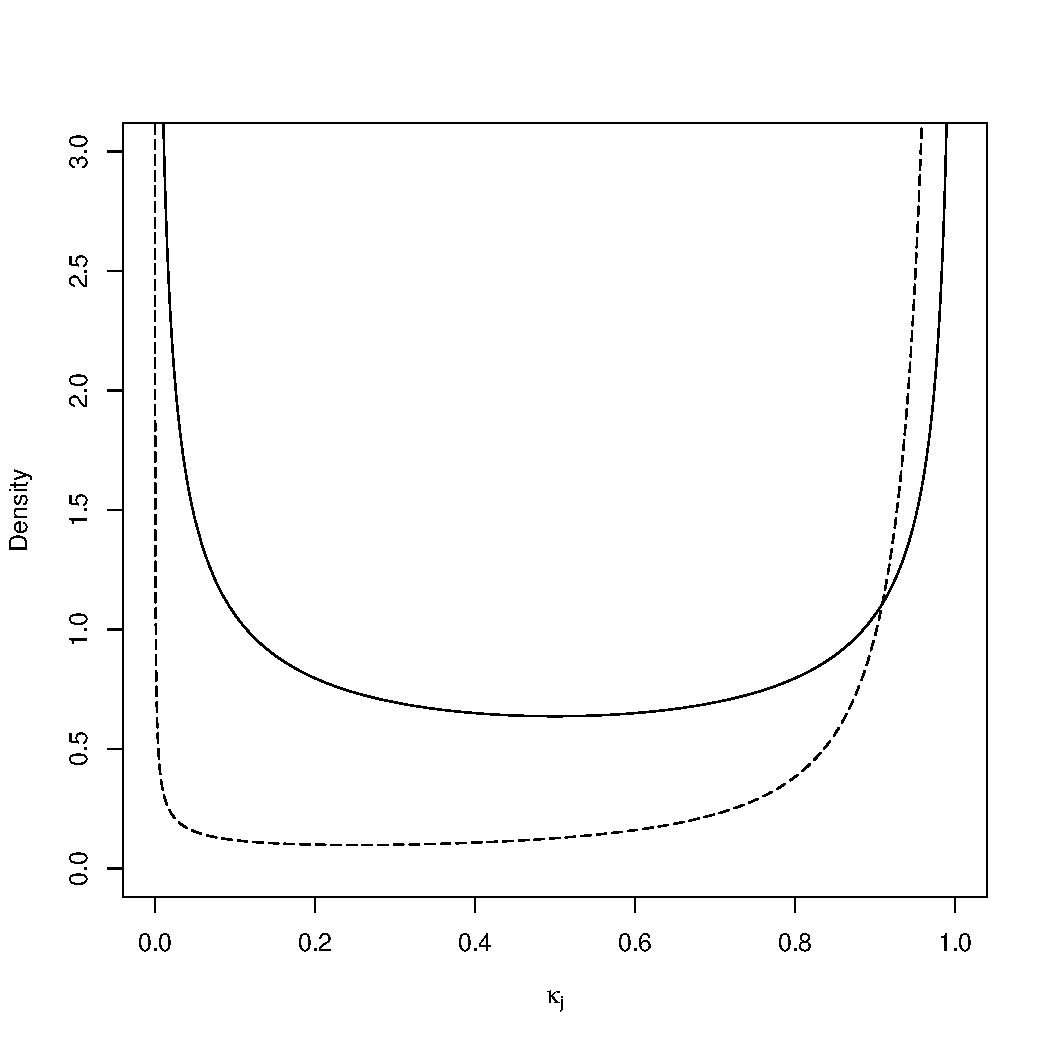
\includegraphics[width=0.5\textwidth]{../plots/kappa.pdf}
 \caption[Conditional density of the shrinkage factor $\kappa_j$]{Conditional density of the shrinkage factor $\kappa_j$ for $n\sigma^{-2}\tau^2 = 1$ (solid) and 
 for $n\sigma^{-2}\tau^2 = 0.1$ (dashed).}
 \label{fig:hs}
\end{figure}
For $n\sigma^{-2}\tau^2 = 1$ it holds that $\kappa_j \sim \text{Beta}(\frac{1}{2},\frac{1}{2})$ and its horseshoe resembling density can be seen in Fig. \ref{fig:hs}, from which the name of this method was derived. While under $n\sigma^{-2}\tau^2 = 1$ equal probability mass is distributed on shrinkage and no shrinkage, under  $n\sigma^{-2}\tau^2 = 0.1$ more mass is distributed towards $1$, which means that shrinkage is favoured.


\subsection{Extending horseshoe prior to the case of grouped variables}
\label{sec:hsg}
In additive models two natural group structures arise:
\begin{enumerate}
\item A categorical predictor with $m_{G_1}$ levels can be modelled with $m_{G_1} -1$ dummy coded variables, which represent a group of $m_{G_1} - 1$ linear predictors.
\item A smoothing function with parameter $\mathbf{u} \in \mathbb{R}^{K_1}$ also can be seen as a group of $K_1$ parameters. 
\end{enumerate}
Because one usually wants a smooth function defined on the whole domain and does not want to select categorical predictors level-wise, the horseshoe prior can be straightforwardly extended for this grouped structures, s.t. for an additive model as defined in Eq. (\ref{eq:am}), where the $g$ linear predictors are categorical with number of levels $m_{G_i}$ and where the parameter vector $\mathbf{u}_j \in \mathbb{R}^{K_j}$ of the $m_s$ smoothing functions,
\begin{align}
\beta|\; \sigma^2,\tau^2, \lambda^2_{11},\dots,\lambda^2_{1g} \sim N(0, \sigma^2\tau^2\mathbf{D}_{\lambda_1}),\\
\forall j \in  \{1,\dots,m_s\}\quad \mathbf{u}_j|\; \tau, \lambda_{2j}  \sim N(0, \tau^2\lambda_{2j}^2\mathbf{Z}_j),
\end{align}
where $\mathbf{D}_{\lambda_1} = \text{diag}(\lambda_{11}^2I_{m_{G_1}},\dots,\lambda_{1g}^2I_{m_{G_g}})$ and 
\begin{align*}
\lambda_{1i}|\;\tau \sim \text{C}^+(0,\tau), \quad \lambda_{2i}|\;\tau \sim \text{C}^+(0,\tau), \quad \tau \sim \text{C}^+(0,1).
\end{align*}
This means every group structure has one local shrinkage parameter. Hence the whole group is either shrunken as a whole or stays unshrunken.
\subsection{Hyperprior choice for global shrinkage parameter}
\label{sec:opt}
In [\cite{horseshoe}] it is shown that for the global shrinkage parameter the choice of scale 1 can produce suboptimal results  in settings where $\tau$ can not well be identified by the data, e.g high ratio of number of parameter to number of data or very noisy data. Hence the authors propose to introduce $\tau_0$ as an hyper-parameter, s.t. $\tau \sim \text{C}^+(0,\tau_0)$ and show that an good way to choose this parameter is by using an guess of the number of relevant variables $p_0$ of of all the $D$ to be shrunken variables, s.t.
\begin{equation}
\tau_0 = \frac{p_0}{D-p_0}\frac{\sigma}{\sqrt{n}}.
\label{eq:tau0}
\end{equation}
In this thesis it will be shown, that this choice of $\tau_0$ is still reasonable in the setting of grouped variables as discussed in section \ref{sec:hsg}: \\
Now consider the grouped variables setting of section \ref{sec:hsg}. 
Every group has its own local shrinkage coefficient $\kappa_{ij}$.
From the prior distribution of $\kappa_{ij}$ (\ref{eq:kappa})\footnote{Since the structures of Eq. (\ref{eq:mubeta}) and Eq. (\ref{eq:muU}) are similar and $\mathbf{Z}$ is a diagonal covariance matrix the derivation of $\kappa$ in the setting of a smooth function can be carried out in the same manner as in section (\ref{sec:mfound}).} it follows that
\begin{equation}
\mathbb{E}(\kappa_{ij}|\; \tau, \sigma) = \underbrace{\frac{1}{1+\sigma^{-1}\tau\sqrt{n}}}_{=:\mu_\kappa}.
\end{equation}
Since $\kappa_{ij}$ is typically either near zero or near one it motivates the definition of effective number of parameter $m_{\text{eff}}$ as 
\begin{equation}
m_{\text{eff}} = \sum^g_{i=1}(1-\kappa_{1i})m_{G_i} + \sum^{m_s}_{j=1}(1-\kappa_{2j})K_j.
\label{eq:meff}
\end{equation}
By taking the expectation of Eq. (\ref{eq:meff}) it follows that
\begin{equation}
\mathbb{E}(m_{\text{eff}}|\; \tau, \sigma) = (1-\mu_\kappa)\underbrace{( \sum^g_{i=1}m_{G_i} + \sum^{m_s}_{j=1}K_j)}_{=: D} = \frac{\sigma^{-1}\tau\sqrt{n}}{1+\sigma^{-1}\tau\sqrt{n}}D.
\label{eq:meffg}
\end{equation}
By solving Eq. (\ref{eq:meffg}) for $\tau$ for an guess of the effective number of parameter $p_0$ the same proposal as presented in Eq. (\ref{eq:tau0}) is derived. The suggested integration of $\tau_0$ in the model is done by using $\tau \sim \text{C}^+(0, \tau_0)$, because then the median of $\tau = \tau_0$ and the heavy tails of the half-cauchy distribution allows for a higher adaptivity to the data. The integration can be done in other ways than using $\tau \sim \text{C}^+(0,\tau_0)$, e.g. fixing $\tau$ to $\tau_0$ or using $\tau \sim N^+(0,\tau_0)$. The effects of these other approaches are discussed in [\cite{horseshoe}].
\subsection{Practical aspects}
\label{sec:pract}
When using NUTS (\ref{sec:HMC}) to sample from the posterior distribution of a horseshoe prior model, so-called \textit{divergent transition} can occur (as described in [\cite{paramprob}]), where the step size of the leapfrog integrator is so big that some features of the target distribution can not be depicted, i.e. the estimation becomes biased. To encounter this the general step size can be made smaller or a reparametrization, s.t. the geometry of the posterior distribution is simplified, can be used or both. For this thesis the parametrization as suggested in
[\cite{reparam}](codes at \url{https://github.com/to-mi/stan-survival-shrinkage}) is used, where a parameter $\nu$ with $\nu \sim \text{C}^+(0,v_0)$ is not directly sampled from the half-cauchy distribution, but instead auxiliary parameters $r_1,r_2$ are introduced, s.t. \begin{equation}
\nu = r_1 \sqrt{r_2}.
\end{equation}
When $r_1 \sim N(0,v_0)$ and $r_1 \sim \text{InvG}(0.5,0.5)$ it follows that $\nu \sim \text{C}^+(0,v_0)$. By sampling $\nu$ indirectly with $r_1$ and $r_2$ the number of divergent transition is lowered, but still a relatively small step size is needed. \\

\pagebreak
\section{Simulations}
\label{sec:sim}
To test the capabilities of the grouped horseshoe priors separately two simulation studies are conducted. On the one hand a model only consisting of factor variables is estimated and different choices of the hyperparameter $\tau_0$ are compared in section \ref{sec:lp}, while on the other hand a pure smooth function model is estimated in section \ref{sec:sf} and compared to estimations done by other variable selection methods such as spikeSlabGAM (see [\cite{scheipl}]) and GAMSEL (see [\cite{gamsel}]), where an overlap group-lasso penalty is used. \\
Both simulation studies are special cases of the additive model (\ref{sec:AddMod}). In general when $\mathbf{U}, \mathbf{X}_1,\dots ,\mathbf{X}_{m_s}$ are created by a data generating process (DGP) the "true" predictor $\eta$ can be evaluated for given coefficient vectors $\beta, \gamma_1 ,\dots ,\gamma_{m_s}$ as $\eta = \mathbf{U}\mathbf{\beta} +  \sum^{m_s}_{i=1} \mathbf{X}_i\mathbf{\gamma}_i$ and the response $\mathbf{y}$ as $\mathbf{y} = \eta + \epsilon$. The number of all variables with non zero influence will be denoted as $D$. To control the difficulty of estimating the coefficient vectors and $\eta$ the so-called signal-to-noise ratio SNR is used. The SNR is defined as $\text{SNR} = n \;\text{sd}^2_\eta / \sum^n_{i=1}\epsilon^2_i,$ where $\text{sd}_\eta = \sqrt{\sum^n_{i=1}(\bar{\eta} -\eta_i)^2/n},$ i.e. SNR is the ratio of the systematic variability (\textit{signal}) over the unsystematic one caused by the Gaussian error terms $\epsilon$.
To simulate a certain SNR level the response $\mathbf{y}$ can be sampled as $y_i \sim N(\eta_i , \text{sd}_\eta^2 / \text{SNR})$. \\
For every model 3 different prior specifications are compared:
\begin{itemize}
\item '\textit{strict}' prior with $p_0 = 1$,
\item '\textit{optimal} prior with $p_0 = \;$true number of non zero influence coefficients,
\item '\textit{loose}' prior with $p_0 = D-1$.
\end{itemize}
In this chapter for every prior 4 chains with a size of 500 elements are simulated.
\newpage
\subsection{Linear predictor scenario}
\label{sec:lp}
In this simple setting the shrinkage property of the grouped horseshoe prior is investigated in the case of categorical predictors solely. As a reference a linear model only based on the non-zero influence variables is estimated, which will be referred as the "oracle"-model. The DGP is described in section (\ref{sec:lpdgp}) and the results are discussed in (\ref{sec:lpres}).

\subsubsection{Data generation}
\label{sec:lpdgp}
The DGP of this setting can be described as follows:
\begin{itemize}
\item $n = 100$ observations,
\item $\text{SNR} = 0.1, 1, 5$,
\item 9 categorical variables are defined as $\forall i \in \{1,2,3\}$
\begin{itemize}
\item the '\textit{small-sized}' groups $G_{i1}$ with levels $g_{11},g_{12},g_{13}$,
\item the '\textit{medium-sized}' groups$G_{i2}$ with levels $g_{21},\dots,g_{25}$,
\item the '\textit{large-sized}' groups $G_{i3}$ with levels $g_{31},\dots,g_{39}$,
\end{itemize}
\item the 9 to the $G_{ij}$ associated coefficient vectors are defined as
\begin{itemize}
\item $\beta_{11} = (0,1,2),$ 
\item $\beta_{12} = (0,1,4/3,5/3,2),$ 
\item $\beta_{13} = (0,1,8/7,9/7,\dots2),$ 
\item $\forall i \in \{2,3\}, j \in \{1,2,3\} \;\beta_{ij} = 0,$ 
\end{itemize}
\item two subscenarios are defined as
\begin{itemize}
\item a '\textit{low sparsity}' scenario: Generate 6 covariates from $G_{i1},G_{i2},G_{i3}$ with $i \in \{1,2\}$, i.e. 3 of which have zero influence, s.t. the true linear predictor is 
\begin{equation*}
\eta = \sum^3_{j=1}\mathbf{1}_{\{g_{1j}\}}(x_1) \cdot \beta_{11,j} +  \sum^5_{j=1}\mathbf{1}_{\{g_{2j}\}}(x_2) \cdot \beta_{12,j} +  
\sum^9_{j=1}\mathbf{1}_{\{g_{3j}\}}(x_3) \cdot \beta_{13,j},
\end{equation*}
\item a '\textit{high sparsity}' scenario: Generate 9 covariates from $G_{i1},G_{i2},G_{i3}$ with $i \in \{1,2,3\}$, i.e. 6 of which have zero influence, s.t. the true linear predictor remains as
\begin{equation*}
\eta = \sum^3_{j=1}\mathbf{1}_{\{g_{1j}\}}(x_1) \cdot \beta_{11,j} +  \sum^5_{j=1}\mathbf{1}_{\{g_{2j}\}}(x_2) \cdot \beta_{12,j} +  
\sum^9_{j=1}\mathbf{1}_{\{g_{3j}\}}(x_3) \cdot \beta_{13,j},
\end{equation*}
\end{itemize}
\item 100 replication per setting.
\end{itemize}
The predictive MSE is evaluated on test data sets with 5000 observations.
\subsubsection{Results}
\label{sec:lpres}
\begin{figure}[hbt!]
 \centering
 \includegraphics[width=0.65\textwidth]{../plots/lp-mse.pdf}
 \caption[MSE / OracleMSE (linear predictor scenario)]{MSE / OracleMSE grouped by priors with different level of shrinkage.}
 \label{fig:lp-mse}
\end{figure}
In this simulation study there are two main objectives. Firstly to measure how the strictness of the shrinkage effects the overall quality and secondly if the shrinkage is influenced by the size of the groups. The coefficient vectors have been scaled, s.t. they span the same interval, in order of making the groups comparable. \\
In Fig. (\ref{fig:lp-mse}) it can be seen that the distributions of the MSEs for SNR = 0.1, 5 differ not greatly. Also the different level of sparsity does not seem to have an structural effect on these distributions. Solely for SNR = 1 it can be observed, that with looser shrinkage the MSEs are drawn to slightly smaller values. \\ 
When comparing the combined MSEs of all groups of the coefficient vectors only for SNR = 0.1, 1 with looser shrinkage the MSEs of the non-zero influence parameter gets smaller and the MSE of the zero influence variables rises minimally as one can observe in Fig. (\ref{fig:lp-pmse-ov}). For small-sized groups an effect on the MSE of the parameter estimate can only be observed for SNR = 0.1, where in Fig. (\ref{fig:lp-pmse-small}) it is seen that while for the low sparsity scenario the parameter MSE exhibits the same behaviour as the combined one for the high sparsity scenario the optimal prior seems to performs slightly better in terms of the MSE. 
It can be observed that for SNR = 1 the MSEs of the medium-sized groups have a wider but lower variance in Fig (\ref{fig:lp-pmse-medium}) than the combined ones. For the large-sized groups as seen in Fig. (\ref{fig:lp-pmse-large}) seemingly exhibits the same structure as displayed in Fig. (\ref{fig:lp-pmse-ov})  of the combined MSEs. \\ By comparing all figures of Fig. (\ref{fig:lp-pmse}) it can be concluded that for $\text{SNR} \geq 5$ the strictness of the prior impacts lesser the MSEs and with a higher SNR the MSEs of the parameter estimates get smaller. Also it can be stated that while the size of the group has an effect on the performance in nearly all settings the level of sparsity has only an minor effect in some cases, i.e. the grouped horseshoe priors appears to be quite robust against different levels of sparsity.

\begin{figure}[pbt!]
 \centering
\begin{subfigure}[b]{0.49\textwidth}
 \includegraphics[width=\textwidth]{../plots/lp-paramMSEoverall.pdf}
 \caption{Combined MSE of all groups of parameter estimate grouped by priors with different level of shrinkage.}
 \label{fig:lp-pmse-ov}
\end{subfigure} \hfill
\begin{subfigure}[b]{0.49\textwidth}
 \includegraphics[width=\textwidth]{../plots/lp-paramMSEsmall.pdf}
 \caption{MSE of parameter estimate of the small groups grouped by priors with different level of shrinkage.}
 \label{fig:lp-pmse-small}
 \end{subfigure}
 \begin{subfigure}[b]{0.49\textwidth}
 \includegraphics[width=\textwidth]{../plots/lp-paramMSEmedium.pdf}
 \caption{MSE of parameter estimate of the medium groups grouped by priors with different level of shrinkage.}
 \label{fig:lp-pmse-medium}
\end{subfigure} \hfill
\begin{subfigure}[b]{0.49\textwidth}
 \includegraphics[width=\textwidth]{../plots/lp-paramMSElarge.pdf}
 \caption{MSE of parameter estimates of the large groups grouped by priors with different level of shrinkage.}
 \label{fig:lp-pmse-large}
 \end{subfigure}
\end{figure}
\begin{figure}[pbt!]\ContinuedFloat
 \centering
 \caption[MSE of parameter estimates]{MSE of parameter estimate grouped by priors with different level of shrinkage.}
 \label{fig:lp-pmse}
\end{figure}

\FloatBarrier
\subsection{Smooth functions scenario}
In order of testing the performance of the grouped horseshoe priors in the setting of smooth functions the simulation study in 4.1.5 of [\cite{scheipl}] is replicated. As a reference a conventional GAM (as implemented in [\cite{gam}]) only based on the non-zero influence variables is estimated, which will be referred as the "oracle"-model. The performance is compared with a Bayesian alternative model approach spikeSlabGAM (see [\cite{scheipl}]) and the non Bayesian inference based method GAMSEL (see [\cite{gamsel}]). The DGP is described in section (\ref{sec:sfdgp}) and the results are discussed in (\ref{sec:sfres}).
%oracle %D
\label{sec:sf}
\subsubsection{Data generation}
The DGP of this setting can be described as follows:
\begin{itemize}
\item $n = 200$ observations,
\item $\text{SNR} = 5, 20$,
\item 4 functions, which enter the linear predictor, are defined as
\begin{itemize}
\item $f_1(x) = x,$
\item $f_2(x) = x + \frac{(2x-2)^2}{5.5},$
\item $f_3(x) = -x + \pi\sin(\pi x),$
\item $f_4(x) = 0.5x + 1.5\phi(2(x-0.2))-\phi(x+0.4)$, where $\phi$ is the standard normal density function.
\end{itemize}
\item two subscenarios are defined as
\begin{itemize}
\item a '\textit{low sparsity}' scenario: Generate 16 covariates, 12 of which have non-zero influence, s.t. the true linear predictor is 
\begin{align*}
\eta & = f_1(x_1) + f_2(x_2) + f_3(x_3) + f_4(x_4) + \\
& + 1.5( f_1(x_5) + f_2(x_6) + f_3(x_7) + f_4(x_8)) + \\ 
& + 2(f_1(x_9) + f_2(x_{10}) + f_3(x_{11}) + f_4(x_{12})) ).
\end{align*}
\item a '\textit{low sparsity}' scenario: Generate 20 covariates, 4 of which have non-zero influence, s.t. the true linear predictor is 
\begin{equation*}
\eta = f_1(x_1) + f_2(x_2) + f_3(x_3) + f_4(x_4). 
\end{equation*}
\end{itemize}
\item The covariates are either 
\begin{itemize}
\item $\overset{\text{i.i.d.}}{\sim} \mathcal{U}[-2,2]$ or 
\item from an $\text{AR}(1)$ process with correlation $\rho = 0.7$.
\end{itemize}
\item 100 replications per setting.
\end{itemize}
The predictive MSE is evaluated on test data sets with 5000 observations.
\label{sec:sfdgp}
\subsubsection{Results}
\label{sec:sfres}
\begin{figure}[hbt!]
 \centering
\begin{subfigure}[b]{0.49\textwidth}
 \includegraphics[width=\textwidth]{../plots/sf-msea.pdf}
\caption {MSE / OracleMSE grouped by priors with different level of shrinkage with limited y-axis.}
 \label{fig:sf-msea}
\end{subfigure}\hfill
\begin{subfigure}[b]{0.49\textwidth}
 \includegraphics[width=\textwidth]{../plots/sf-mseb.pdf}
\caption {MSE / OracleMSE grouped by priors with different level of shrinkage with all data points.}
 \label{fig:sf-mseb}
 \end{subfigure}
 \caption[MSE / OracleMSE (smooth functions scenario)]{MSE / OracleMSE grouped by priors.}
  \label{fig:sf-mse}
\end{figure} 
In this section grouped horseshoe priors with different levels of shrinkage  are compared to each other, spikeSlabGAM, and GAMSEL in the smooth functions setting. For the horseshoe priors and spikeSlabGAM every covariate is fitted with a p-spline of order 2 and degree 3 with 20 knots. Default setting consisting of 3 chains of length 500 are used for spikeSlabGAM. For GAMSEL splines of degree 6 with nominal number of basis elements of 10 are fitted. The regularization parameter $\lambda$ of GAMSEL is chosen from 50 10-fold cross validations. It is also evaluated how well the function approximation is carried out by the different priors. 
In Fig. (\ref{fig:sf-msea}) it can be seen that the level of shrinkage does not seem to effect the performance in terms of the MSE of the grouped horseshoe priors.
Also it can be observed that the grouped horseshoe priors perform quite robust compared to the other methods. Especially in the case of correlated covariates this can be noticed, where in the low sparsity scenario the MSEs of the horseshoe priors are lower distributed than the MSEs of spikeSlabGAM. In the other cases spikeSlabGAM performs slightly better than the horseshoe priors. For this simulation GAMSEL performs in terms of MSE far worse as it can be seen in Fig. (\ref{fig:sf-mseb}), e.g many extreme high values, except for uncorrelated covariates, where for SNR = 5 it has a clearly better performance in both sparsity scenarios. 
The MSEs of the centered function output estimates seem to have no noteworthy differences for different levels of shrinkage as it can be verified in Fig. (\ref{fig:sf-quality}), except for a slightly better performance of the more loose shrinkage for SNR = 5 and $\rho = 0.7$. Which coincides with the MSE distribution of the different shrinkage levels observed in Fig. (\ref{fig:sf-mse}).
\begin{figure}[hbt!]
 \centering
 \includegraphics[width=0.65\textwidth]{../plots/sf-quality.pdf}
 \caption{MSE of function output estimate.}
 \label{fig:sf-quality}
\end{figure}
\FloatBarrier
\pagebreak

\section{Benchmarking}
\label{sec:benchmark}
In this chapter the methods of section (\ref{sec:sim}) are applied on real data sets and their performance is compared. Both data sets are modeled as Gaussian, i.e. the output is numerical and the error terms are assumed to be normal distributed. In section (\ref{sec:am}) the output is estimated based only on categorical predictors and in section (\ref{sec:bn}) smooth functions are estimated for all numerical input variables. In this chapter the number of all coefficients will be denoted as $D$.
\subsection{Automobile}
\label{sec:am}
This data set is from the Univerisity of California Irvine Machine Learning Repository [\cite{uci}]. The data was compiled by Jeffrey C. Schlimmer from the following sources:
\begin{itemize}
\item 1985 Model Import Car and Truck Specifications, 1985 Ward's Automotive Yearbook.
\item Personal Auto Manuals, Insurance Services Office, 160 Water Street, New York, NY 10038
\item Insurance Collision Report, Insurance Institute for Highway Safety, Watergate 600, Washington, DC 20037
\end{itemize}
In this data set information of different cars and their price, as described in section (\ref{sec:amdd}), is contained. The performance of estimating the price based on only the categorical predictors is evaluated in section (\ref{sec:amcs}).
\subsubsection{Data description and modifications}
\label{sec:amdd}
The automobile data set consists of 205 observations with 26 attributes. Of these 26 attributes only the 10 nominal predictors are selected, s.t. the performance can be compared with the gglasso method (see [\cite{gglasso}]). The numerical outcome variable of interest is the price of the car, which ranges from 5118 to 45400\$. \\The nominal predictors for the price of one car are the make with 22 different kinds, whether it runs on diesel or gas, whether its engine is naturally aspirated or turbocharged, if  it has two or four doors, the car body design with 5 different kinds, whether is has front-wheel drive, back-wheel drive or four-wheel drive, whether the engine is located in the front or the rear, different engine-types with 7 different kinds, the number of cylinder modeled as categorical variable with 7 types, the fuel system with 8 different kinds. Only complete cases are used, s.t. only 199 observation are used for the estimation of the models.\\ \\
To create two levels of artificial sparsity in the data the 10 predictors are 1-times/2-times duplicated, permutated and added to the data set, s.t. the newly added data is distributed like the original data, but without relation to the outcome.
\subsubsection{Comparisions and Results}
\label{sec:amcs}
\begin{figure}[hbt!]
 \centering
 \includegraphics[width=0.65\textwidth]{../plots/am-mse.pdf}
 \caption[RMSE of prediction (automobile)]{RMSE of prediction of 50 shuffle splits.}
 \label{fig:am-mse}
\end{figure}
For this simulation 3 different horseshoe priors are evaluated with $p_0 = 0.1D, 0.25D, 0.5D$ (note, that $D$ changes with added sparsity).  For every prior 4 chains with a size of 200 elements are simulated. Default setting consisting of 3 chains of length 500 are used for spikeSlabGAM. The regularization parameter $\lambda$ of gglasso is chosen from 100 5-fold cross validations.
The performance of these methods is compared with their RMSEs, which are drawn from 50 valid\footnote{A split is accepted, if the test data contains only  levels, which are also present in the training data.}  shuffle splits, i.e. 50 times the data set is randomly divided into training and test data with ratio 4:1. \\
In Fig. (\ref{fig:am-mse}) it can be observed that the horseshoe priors differ only slightly for all levels of shrinkage.
Since for the unaltered data the RMSEs of the grouped horseshoe priors and the linear model follow a similar distribution, it is assumed that the data is not sparse. All methods seem to be robust against higher levels of sparsity, except for the linear model as one would expect. For this data set the groups horseshoe priors perfom best in terms of the RMSE, followed by gglasso. The spikeSlabGAM method seems to overestimate the sparsity, which could be a reason the larger RMSE values.
\FloatBarrier
\subsection{Boston housing}
\label{sec:bn}
The data have been taken from the UCI Repository Of Machine Learning Databases [\cite{uci}] and are based on [\cite{boston}]. In this data set information of owner-occupied homes and their neighbourhood in suburbs of Boston and their median value, as described in section (\ref{sec:bndd}), is contained. The performance of estimating the median value based on only the numerical predictors is evaluated in section (\ref{sec:bncs}). 
\subsubsection{Data description and modifications}
The Boston housing data set consists of 506 observations with 14 attributes. Of these 14 attributes only the 12 continuous predictors are selected, s.t. the performance can be compared with the GAMSEL method (see [\cite{gamsel}]). The numerical outcome variable of interest is the median value of owner-occupied homes in \$1000, which ranges from 5 to 50.  \\
The continuous predictors for the median value of owner-occupied homes are the per capita crime rate by town, the proportion of residential land zoned for lots over 25,000 sq.ft., the proportion of non-retail business acres per town, 
the nitrogen oxides concentration, the average number of rooms per dwelling, 
proportion of owner-occupied units built prior to 1940, weighted mean of distances to five Boston employment centres, full-value property-tax rate, 
pupil-teacher ratio by town, the proportion of African-American by town, the lower status of the population. \\
To create an artificial sparsity in the data the 12 predictors are duplicated, permutated and added to the data set, s.t. the newly added data is distributed like the original data, but without relation to the outcome.
\label{sec:bndd}
\subsubsection{Comparisions and Results}
\label{sec:bncs}
\begin{figure}[hbt!]
 \centering
\begin{subfigure}[b]{0.49\textwidth}
 \includegraphics[width=1\textwidth]{../plots/bn-msea.pdf}
\caption {RMSE of prediction of 10 times repeated 5-fold cross validation with limited y-axis.}
 \label{fig:bn-msea}
\end{subfigure}\hfill
\begin{subfigure}[b]{0.49\textwidth}
 \includegraphics[width=1\textwidth]{../plots/bn-mseb.pdf}
\caption {RMSE of prediction of 10 times repeated 5-fold cross validation with all data points.}
 \label{fig:bn-mseb}
 \end{subfigure}
 \caption[RMSE of prediction (Boston housing)]{RMSE of prediction of 10 times repeated 5-fold cross validation.}
 \label{fig:bn-mse}
\end{figure}
For this simulation 3 different horseshoe priors are evaluated with $p_0 = 0.1D, 0.2D, 0.4D$ (note, that $D$ changes with added sparsity).  For every prior 4 chains with a size of 100 elements are simulated. Default setting consisting of 3 chains of length 500 are used for spikeSlabGAM. For GAMSEL splines of maximum number of spline basis function of 10 with a degree of freedom of 5 are fitted. The regularization parameter $\lambda$ of GAMSEL is chosen from 50 10-fold cross validations. Also for reference a linear model and GAM with splines of degree 6 are fitted.  \\
The performance of these methods is compared with their RMSEs, which are drawn from 10 5-fold cross validations. \\
Since the GAM performs better in terms of RMSE than the linear model as it can be seen in Fig. (\ref{fig:bn-msea}) it can be concluded that there are non-linear effects in the data. In this setting spikeSlabGAM has the lowest RMSE values, which are nearly followed by the RMSE values of the GAM, for both levels of sparsity. The horseshoe priors perform slightly worse than spikeSlabGAM, but still robust. No difference can be noted for the different levels of shrinkage. GAMSEL has a similar performance than the grouped horseshoe priors in this data set, but with some far higher extreme values as it can be seen in Fig. (\ref{fig:bn-mseb}).
\FloatBarrier
\section{Conclusions}
As this thesis shows the grouped horseshoe priors are able to estimate robustly point estimates. It is especially robust comparably to the other presented methods against different levels of sparsity as it can be seen in the simulation study (\ref{sec:sf}) and the benchmarks (\ref{sec:benchmark}).
The linear predictor simulation (\ref{sec:lp}) suggests that there is an influence of the size of the groups, which should be investigated further. For this thesis the parametrization $u$ of $\gamma$ as shown in section (\ref{sec:AddMod}) was used. The influence of choosing an other parametrization could be investigated. Also more studies could be done of when a chain is sufficiently long for a good point estimate, since it could be shown in (\ref{sec:am}) that chains of only length 100 produced competitive results. In most cases the hyperparameter choice did not effect the performance in terms of predictive MSE, but in some data situations the \textit{optimal} prior offered a good comprise between estimation error of the zero and non-zero influence variables, as it could be seen in section (\ref{sec:lp}).\\
Also it must be noted that a drawback of using the full Bayesian Inference is that it is quite time-consuming as compared to frequentist methods like gglasso or GAMSEL.  \\
Overall the results of the grouped horseshoe priors look promising and more work should be invested in extending it to the general additive model case and to a broader family of smooth functions. 
\pagebreak
\section{Appendix - Stan code} 
%\subsection{Other variable selection methods}
%\subsubsection{spikeSlabGAM variable selection}
%\subsubsection{Feature selection using LASSO}
%\pagebreak
\subsection{Linear predictor}
\lstinputlisting{../src/ghs-lp.stan}
\pagebreak
\subsection{Smooth functions}
\lstinputlisting{../src/ghs-pspline1D.stan}
\pagebreak

\pagestyle{fancy}
\bibliographystyle{apalike}
\bibliography{thesis} 

\nocite{*} 
\addcontentsline{toc}{section}{Bibliography}
\clearpage

\listoffigures
\addcontentsline{toc}{section}{List of Figures}
\clearpage


\section*{List of Abbreviations}
\addcontentsline{toc}{section}{List of Abbreviations}
\begin{multicols}{2}
  \begin{acronym}[abr]
    \acro{HMC}{Hamiltonian Monte Carlo}
    \acro{NUTS}{No-U-Turn Sampler}    
    \acro{HDP}{highest posterior density}       
    \acro{PLS}{penalized least-squares}
    \acro{DGP}{data generating process}
    \acro{SNR}{signal-to-noise ratio}
    \acro{MSE}{mean squared error}
    \acro{RMSE}{root-mean-square error }   
  \end{acronym}
\end{multicols}



\pagebreak
\subsection*{Statement}
\label{erklaerung}
\vspace*{0.5cm}
I hereby declare that this thesis is my own original work and that all sources have been acknowledged.\\[1.0cm]
Munich, \today \\[2.0cm]
\rule{6.0cm}{0.4pt} \\
Tobias Pielok


\end{document}
